\documentclass{beamer}

\usepackage[utf8]{inputenc} % Включаем поддержку UTF8  
\usepackage[russian]{babel} % Включаем пакет для поддержки русского языка 

\title[Spherical Principal Component Analysis]{Spherical Principal Component Analysis}

\subtitle{Applying spherical PCA algorithm for dimensionality reduction set of unit vectors}

\author[] { Курбет Игорь, Малашенко Сергей }

\date[]{OZON Masters, December 2020}

\begin{document}

\frame{\titlepage}

\begin{frame}
\frametitle{Постановка задачи}
\begin{itemize}
 \item В задачах классификации и распознавания объектов хорошо себе зарекомендовали модели \cite{deng2019arcface}, которые оценивают близость 
 $$X_i \in S^n = \{ x \in \mathbb{R}^{n+1} : \left\lVert x \right\rVert=1 \}$$
 \item В работе предлагается снизить размерность $n$ при помощи метода главных компонент на сфере $S^n \Rightarrow S^m$, где $m < n$.
 \item Качество алгоритма оценивается решением задачи кластеризации векторов $X_i \in S^n, \tilde{X_i} \in S^m$ \cite{4e952c207c0444a9a0083fa9cf4e3cde} в предположении, что $$X_i \sim \sum_{i=1}^{N}\pi_i \mathbb{V}_{n+1}(x | \mu_i, \kappa_i), \mathbb{V}_d(x | \mu_i, \kappa_i)=\frac{\kappa^{\frac{d}{2}-1}}{(2\pi)^{\frac{d}{2}}J_{\frac{d}{2}-1}(\kappa)} e^{\kappa \mu^{\top} x}$$
\end{itemize}
\end{frame}

\begin{frame}
\frametitle{Решение задачи}
Решение общей задачи разбивается на три подзадачи
\begin{itemize}
 \item Разработка и сравнение моделей классификации на наборе данных MNIST. Модели строятся с использованием $SoftMax + NLL$, и $ArcFace$. Для функции потерь $ArcFace$ результатом будет совокупность $X_i$ на тестовой выборке
\item Разработка инструмента, который реализует метод главных компонент на сфере $X_i \in S^n, \tilde{X_i} \in S^m$
\item Разработка инструмента, который решает задачу кластеризации векторов на сфере
\end{itemize}

\end{frame}

\begin{frame}
\frametitle{Модель классификации}
\begin{center}
\includegraphics[scale=0.3]{mnist_model.png}
\end{center}
\begin{align*}
L_{softmax} &= -\frac{1}{N}\sum^{N}_{i=1}\log\frac{e^{W^{T}_{y_{i}}x_{i} + b_{y_{j}} }}{\sum^{N}_{j=1}e^{W^{T}_{j}x + b_j }} \\
L_{arcface} &= -\frac{1}{N}\sum^{N}_{i=1}\log\frac{e^{s\left(\cos\left(\theta_{y_{i}} + m\right)\right)}}{e^{s\left(\cos\left(\theta_{y_{i}} + m\right)\right)} + \sum^{n}_{j=1, j \neq y_{i}}e^{s\cos\theta_{j}}}
\end{align*}
\end{frame}

\begin{frame}
\frametitle{Модель классификации}
\begin{center}
\includegraphics[scale=0.25]{arcface_loss.png}
\end{center}
\begin{align*}
L_{softmax} &= -\frac{1}{N}\sum^{N}_{i=1}\log\frac{e^{W^{T}_{y_{i}}x_{i} + b_{y_{j}} }}{\sum^{N}_{j=1}e^{W^{T}_{j}x + b_j }} \\
L_{arcface} &= -\frac{1}{N}\sum^{N}_{i=1}\log\frac{e^{s\left(\cos\left(\theta_{y_{i}} + m\right)\right)}}{e^{s\left(\cos\left(\theta_{y_{i}} + m\right)\right)} + \sum^{n}_{j=1, j \neq y_{i}}e^{s\cos\theta_{j}}}
\end{align*}
\end{frame}


\begin{frame}
\frametitle{Модель классификации}
\begin{center}
\includegraphics[scale=0.3]{mnist_vgg8_3d.png}
\includegraphics[scale=0.3]{mnist_vgg8_arcface_3d.png}
\end{center}
\begin{center}
\includegraphics[scale=0.3]{mnist_accuracy.png}
\includegraphics[scale=0.3]{mnist_losses.png}
\end{center}
\end{frame}


\begin{frame}
\frametitle{Метод главных компонент на сфере}
\begin{center}
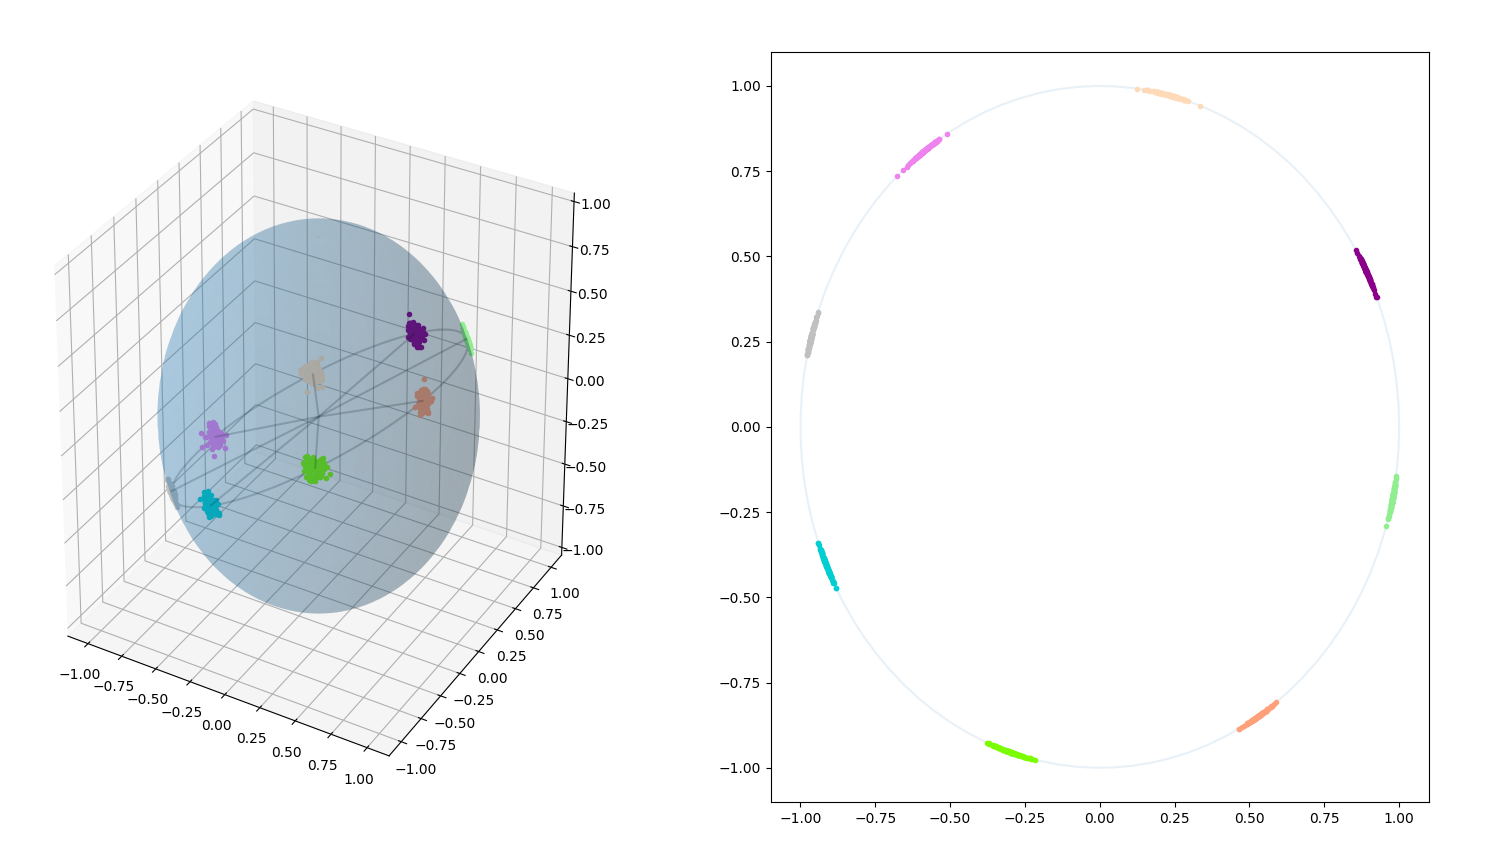
\includegraphics[scale=0.17]{sphericalPCA.png}
\end{center}

$$\underset{\mathrm{U} \in \mathbb{R}^{m x r}, \mathrm{V} \in \mathbb{R}^{r x n} }{minimize} \lVert \mathrm{X - UV} \rVert^2_F, \mathrm{U} \in \mathbb{U}, \mathrm{V} \in \mathbb{V}$$
$$\mathbb{U} = \{\mathrm{U : U^{\top}U=I }\}, \mathbb{V} = \{ \lVert \mathrm{v_j} \rVert = 1, \forall j \}$$
\end{frame}

\begin{frame}[t]
\frametitle{Метод главных компонент на сфере}
\begin{align*}
\onslide<1->{
\mathrm{U(k+1)} &= \underset{\mathrm{U} \in \mathbb{U} }{argmin}{\lVert \mathrm{X - UV(k)} \rVert^2_F} \\ 
\mathrm{v_j(k+1)} &= \underset{\lVert \mathrm{v} \rVert = 1}{argmin}{\lVert \mathrm{x_j - U(k+1)v} \rVert^2_2, \forall j} \\
}
\onslide<2->{
\\
\mathrm{h(U,V)} &= \lVert \mathrm{X - UV} \rVert^2_F = \sum_{j=1}^n \lVert \mathrm{x_j - Uv_j} \rVert^2 \\
\mathrm{U(k+1)} &= \underset{\mathrm{U} \in \mathbb{U} }{argmin}{ \langle \mathrm{U-U(k), \nabla_Uh(U(k),V(k))} \rangle + \frac{\mu}{2} \lVert \mathrm{U - U(k)} \rVert^2_F } \\ 
\mathrm{v_j(k+1)} &= \underset{\lVert \mathrm{v} \rVert = 1}{argmin}{ \langle v- v_j(k), \nabla_{v_j} h(U(k+1),V(k)) \rangle + \frac{\lambda}{2} \lVert \mathrm{v - v_j(k)} \rVert^2 }
}
\end{align*}
\end{frame}

\begin{frame}[t]
\frametitle{Метод главных компонент на сфере}
\begin{align*}
\onslide<1->{
\mathrm{U(k+1)}   &= \underset{\mathrm{U} \in \mathbb{U} }{argmax} \mathrm{ \langle U,2(X-U(k)V(k))V(k)^{\top} \rangle + {\mu}U(k) } \\ 
\mathrm{v_j(k+1)} &= \underset{\lVert \mathrm{v} \rVert = 1}{argmax}\mathrm{\langle v,2U(k+1)^{\top}x_j + (\lambda-2)v_j(k) \rangle} \\
}
\onslide<2->{
\\
\\
\mathrm{U(k+1)}   &= \mathrm{YZ^{\top}, [Y,\Sigma,Z]=svd(2(X-U(k)V(k))V(k)^{\top}) }\\ 
\mathrm{v_j(k+1)} &= \mathrm{ \frac{q}{\lVert q \rVert} }, \mathrm{q=2U(k+1)^{\top} + (\lambda-2)v_j(k)} \\
}
\end{align*}

\end{frame}

\begin{frame}
\frametitle{Кластеризация данных на сфере}
\begin{tabular}{|c|l|l|} 
\hline
\multicolumn{3}{|c|}{Результаты на искусственных данных} \\
\hline
Размерность данных & Точность $\mu$ & Значение $\kappa$  \\ 
\hline
32 & 1.7115e-05 & 14899.34 \\
16 & 2.5601e-05 & 7628.563 \\
8  & 4.3424e-05 &  3212.77 \\
4  & 4.2201e-05 & 464.5948 \\
\hline
\multicolumn{3}{|c|}{Результаты на данных $\mathrm{MNIST}$} \\
\hline
размерность данных & начальная точность & конечная точность \\
\hline
64 -> 24 & 95.33\% & 95.78\% \\
32 -> 9  & 95.29\% & 95.06\% \\
16 -> 8  & 95.03\% & 95.16\% \\
\hline
\end{tabular}
\end{frame}

\begin{frame}
\frametitle{Выводы}
\begin{itemize}
\item Использование нормированных векторов в задачах классификации и распознавания, позволяет повысить качество работы модели.
\item Метод главных компонент на сфере позволяет снизить размерность результирующих векторов, что приводит к повышению локализации кластеров, а также повышению производительности работы общей системы.
\end{itemize}
\end{frame}

\begin{frame}
\frametitle{Перспективы}
\begin{itemize}
\item Опробовать другие распределения, например Power Spherical distribution \cite{decao2020power}
\item Вместо подбора некоторого метапараметра $m$ в функции потерь ArcFace. Решить задачу родственную задаче Томсона на сфере
\end{itemize}
%\includegraphics[scale=0.1]{thomson_proble.gif}
\end{frame}

\begin{frame}[allowframebreaks]
\frametitle{Библография}
\bibliographystyle{amsalpha}
\bibliography{./NumericalLinearAlgebraProject.bib}
\end{frame}


%$$\mathrm{ X_i \sim \sum_{i=1}^{N}\pi_i V_{n+1}(x | \mu_i, \kappa_i), V_d(x | \mu_i, \kappa_i)=\frac{\kappa^{\frac{d}{2}-1}}{(2\pi)^{\frac{d}{2}}J_{\frac{d}{2}-1}(\kappa_i)} e^{\kappa_i {\mu_i}^{\top} x} }$$
\end{document}
